\chapter{RESULTS: GRAPHIC USER INTERFACE}
\label{chap:GUI_results.tex}
\addtocontents{toc}{\protect\setcounter{tocdepth}{1}}
The final GUI is a HTML page generated by the master phyton script. This file is generated by running master script with the asm list files and execution log files as input. The generated .html or .htm file can be viewed by any standard web browser like Internet Explorer, Firefox etc that support JavaScript. As this is just like any other html page with out any dependences, the user can access the page from web as a stand-alone file with out requiring the list files and log files. 
The following figures shows various windows of final GUI.
\section {EXECUTION FLOW GRAPH}
%\figurename{} 
\begin{figure}[H]
\centering
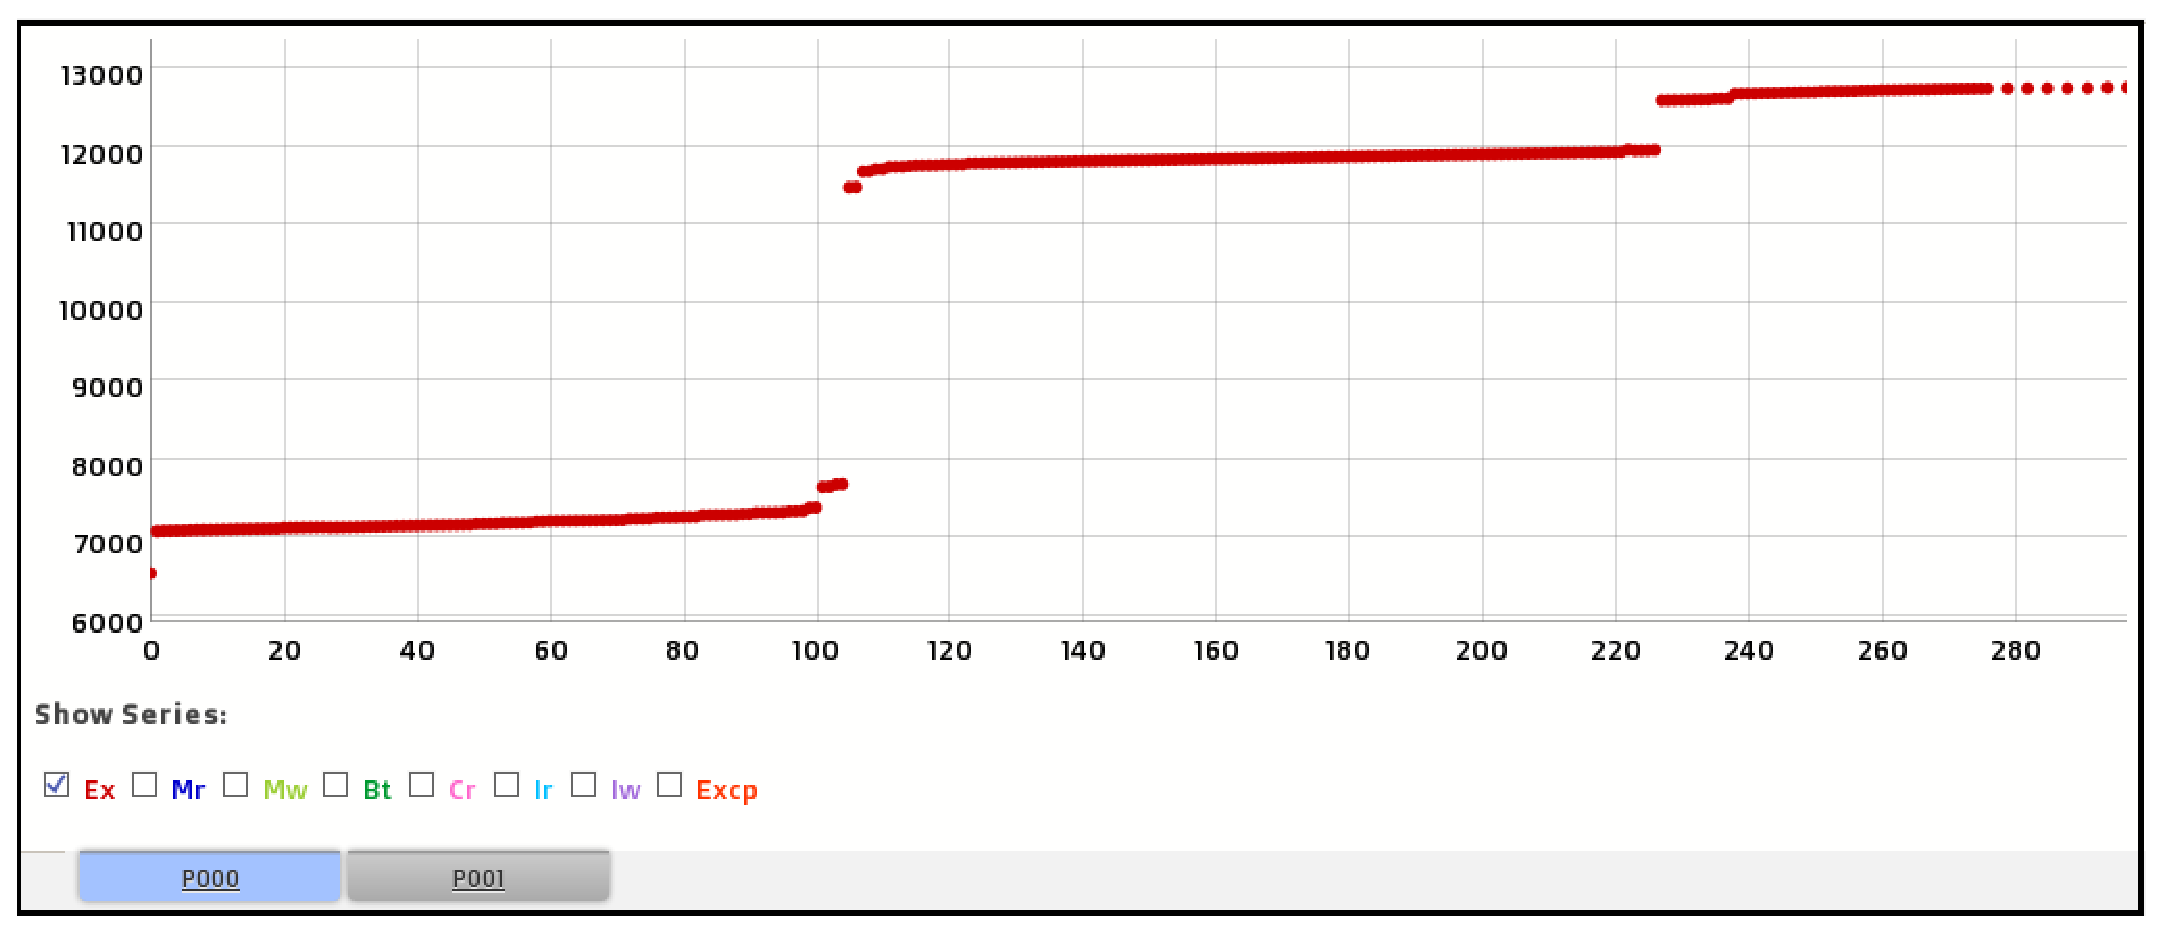
\includegraphics[width=6in]{./figures/gui_graph1.eps}
\caption{Execution Flow Graph}
\label{fig:gui_graph1.eps}
\end{figure}
%\end{tabular}
%\figurename{} 

~\figurename{~\ref{fig:gui_graph1.eps}}shows the main execution flow graph for selected active thread.  
\begin{figure}[H]
\centering
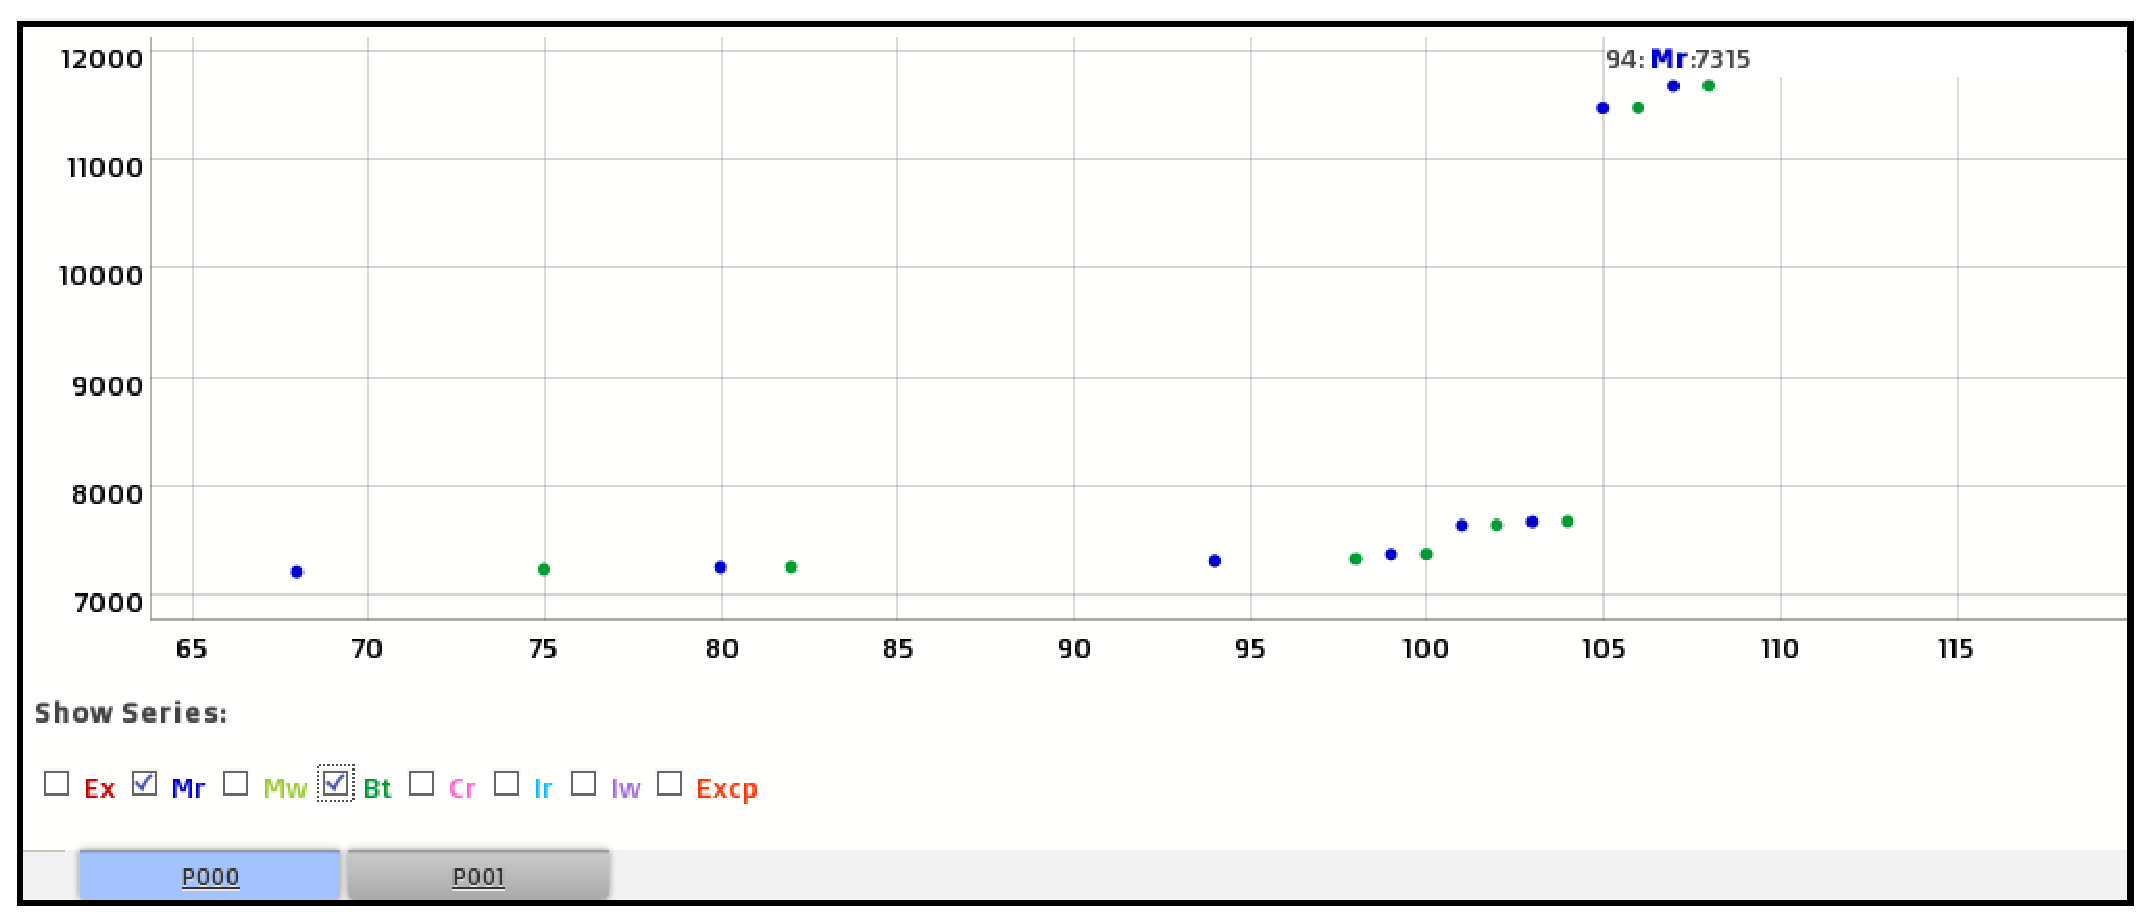
\includegraphics[width=6in]{./figures/gui_graph2.eps}
\caption{Execution Graph With Branching and Memory Writes}
\label{fig:gui_graph2.eps}
\end{figure}
%\end{tabular}
%\figurename{} 

~\figurename{~\ref{fig:gui_graph2.eps}} shows only memory write and branch operation happening in the selected thread.
\section {REGISTER WATCH WINDOW}
\begin{figure}[H]
\centering
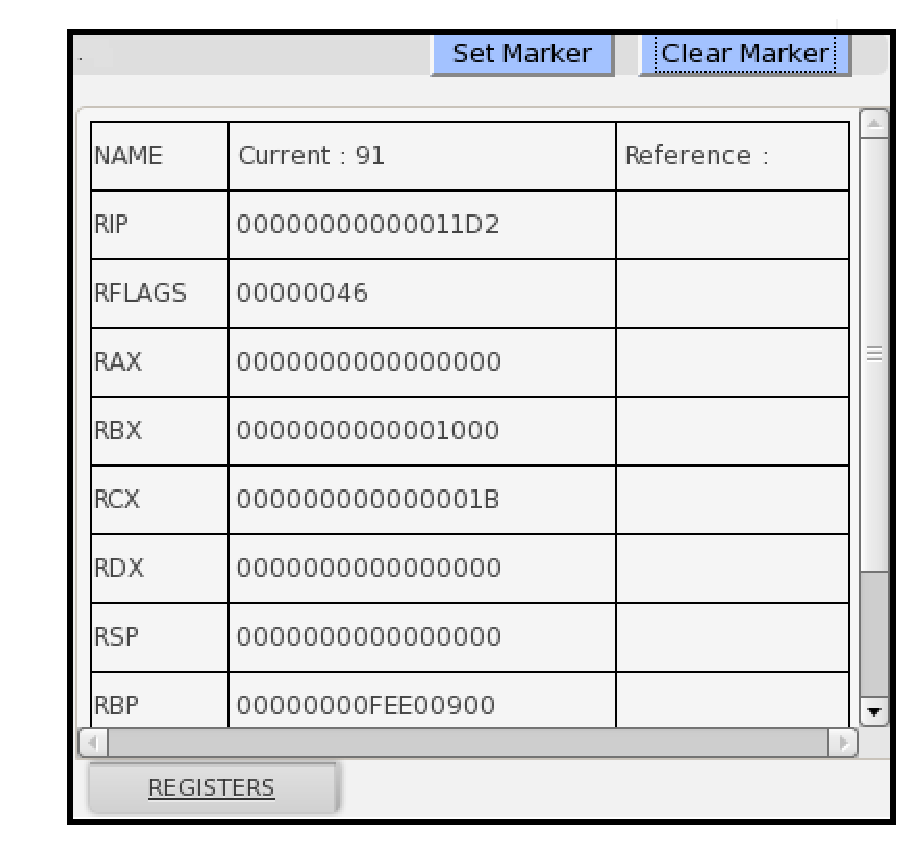
\includegraphics[width=4in, height=2in]{./figures/gui_reg1.eps}
\caption{Register Watch Window}
\label{fig:gui_reg1.eps}
\end{figure}
~\figurename{~\ref{fig:gui_reg1.eps}} shows register window showing updated register values of current selection.
%\end{tabular}
\begin{figure}[H]
\centering
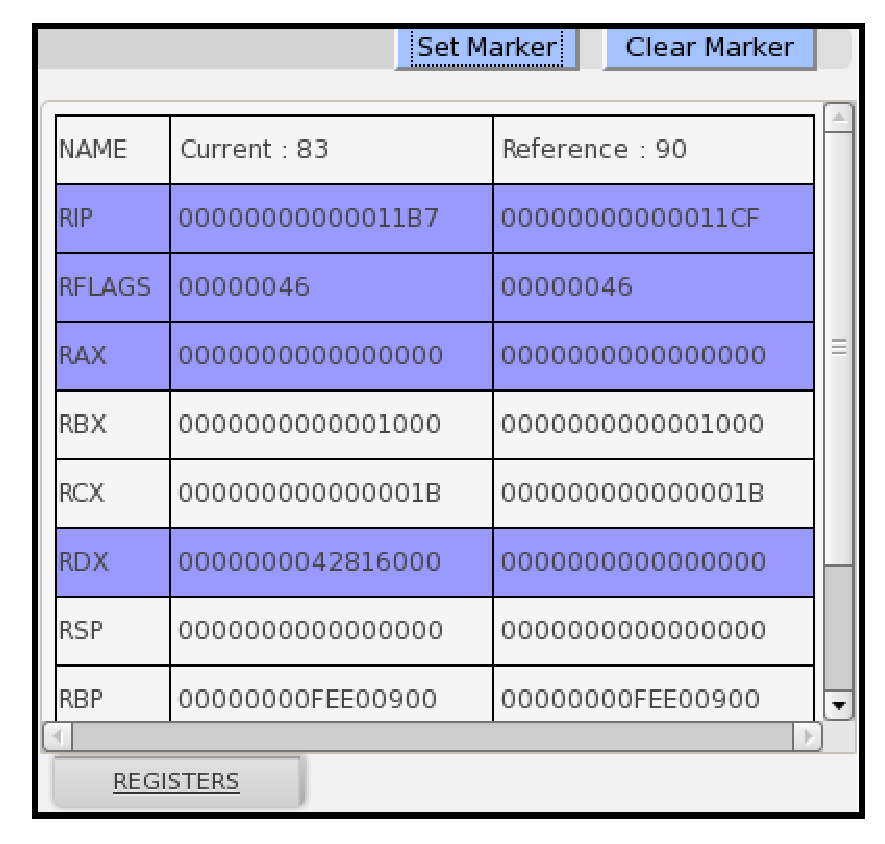
\includegraphics[width=4in, height=2in]{./figures/gui_reg2.eps}
\caption{Register Value Comparison}
\label{fig:gui_reg2.eps}
\end{figure}
%\end{tabular}
~\figurename{~\ref{fig:gui_reg2.eps}} shows the comparison of register states at two different points. Differences are highlighted.
\section {INSTRUCTION WINDOW}
\begin{figure}[H]
\centering
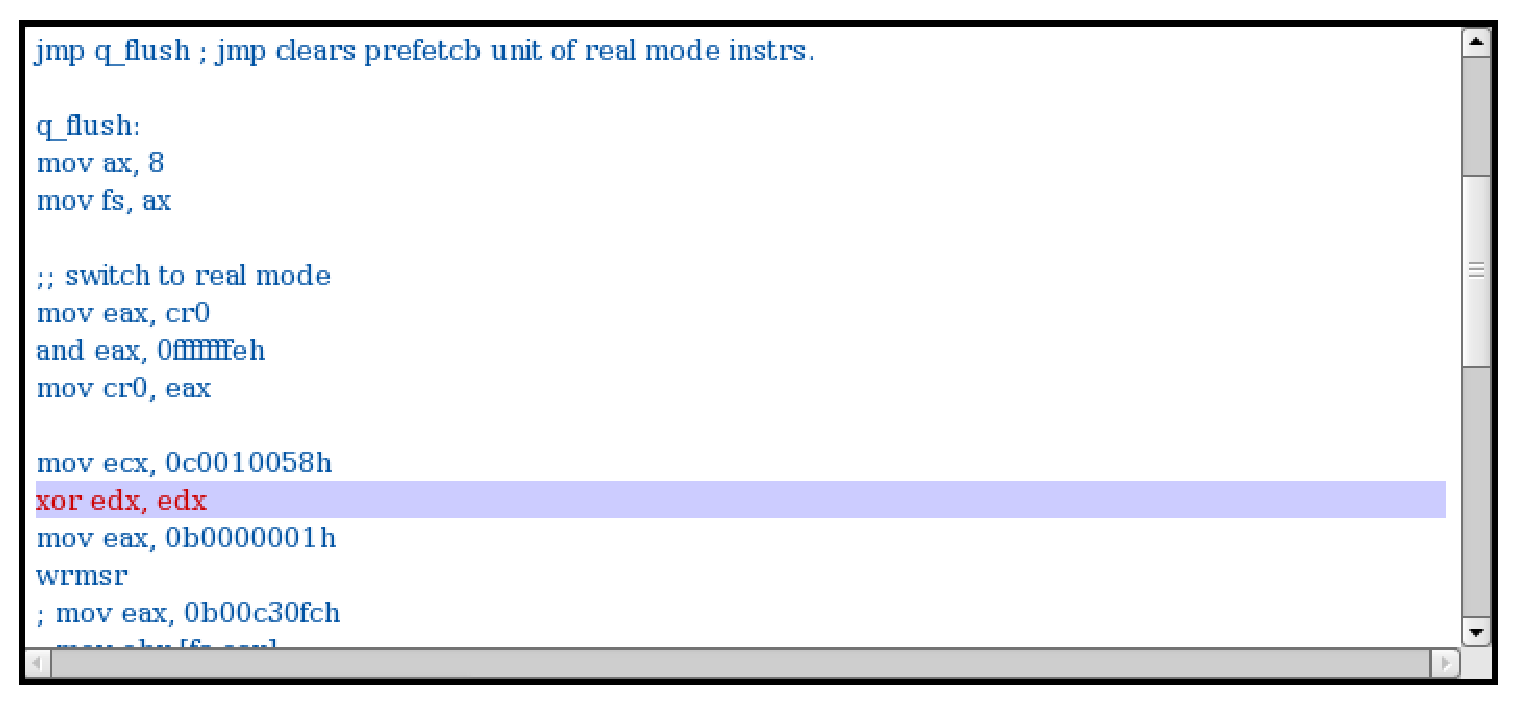
\includegraphics[width=5in, height=3in]{./figures/gui_asm.eps}
\caption{Instruction Window}
\label{fig:gui_asm.eps}
\end{figure}
%\end{tabular}
~\figurename{~\ref{fig:gui_asm.eps}} shows the instruction window which highlights the current selection and also display the context of selected instruction.




































